\documentclass[12pt]{article}
\usepackage[utf8]{inputenc}
\usepackage{float}
\usepackage{amsmath}
\usepackage[tableaux]{prooftrees}
\renewcommand*\linenumberstyle[1]{(#1)}

\usepackage[hmargin=3cm,vmargin=6.0cm]{geometry}
\topmargin=-2cm
\addtolength{\textheight}{6.5cm}
\addtolength{\textwidth}{2.0cm}
\setlength{\oddsidemargin}{0.0cm}
\setlength{\evensidemargin}{0.0cm}
\usepackage{indentfirst}
\usepackage{amsfonts}
\usepackage{tikz}
\usepackage{qtree}
% \usepackage{pmatrix}

\begin{document}

\section*{Student Information}

Name: Kaan Karaçanta \\

ID: 2448546 \\

% Simon’s Algorithm provides an exponential speed-up when determining the period c for functions
% where f : {0, 1}n → {0, 1}n and f(x) = f(y) ←→ x = y ⊕ c.
\section*{Part 1}

% The functions defined are generally two-to-one. Give a specific c that would make the function one-to-one.
\subsection*{\text{a)}}

For this function, $ c = 0^n $ would make it one-to-one.

% What is the minimum number of evaluations required for classical approach to determine whether the function is two-to-one or one-to-one for n = 7.
\subsection*{\text{b)}}

The minimum number of evaluations required to determine exactly whether the function is two-to-one or one-to-one is $ 2^{n-1} + 1 $, so 65. 

% For the following function where n = 3, what is c? Explain your approach for finding c.
\subsection*{\text{c)}}

This is a two-to-one function, $ 000 $ and $ 011 $ are one pair of inputs giving the same result, their xor is $ 011 $, so $ c = 011 $. This relationship can be seen on any other pair of inputs giving the same result.

% Assume you run the circuit 8 times and get the following results for a function with n = 6;
% ’001000’: 1
% ’111111’: 1
% ’000100’: 1
% ’110010’: 2
% ’100110’: 1
% ’000001’: 1
% ’010100’: 1
% Can c be determined with these inputs? If yes, show your calculations step-by-step; if no, explain
% your reasoning.
\subsection*{\text{d)}}

Without knowledge of which specific inputs correspond to the output measurements, we cannot directly determine the secret string c. Simon's algorithm relies on finding n linearly independent equations that result from measuring the quantum state after applying the quantum oracle and subsequent Hadamard gates. These equations are derived from the bitstrings that are guaranteed to be orthogonal to the secret string c.

In this case, while we have 8 measurements with 7 different results, which should theoretically be more than enough for an n=6 bit string, they do not form a set of linearly independent equations. The lack of linear independence means that the measurements do not span the full vector space and therefore do not provide a complete basis to solve for c. 
\\


*This answer is wrong it can be found.

% Provide the circuit for Simon’s Algorithm where n = 4 and c =′ 1010′. Briefly explain the circuit.
% What would you change in the circuit if c is changed to ′0101′?
\subsection*{\text{e)}}

\begin{figure}[H]
    \centering
    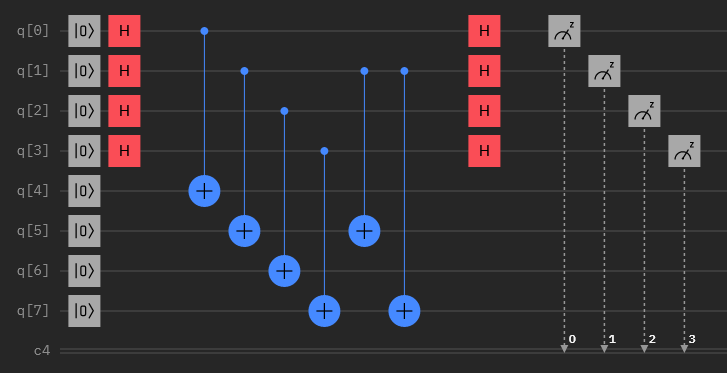
\includegraphics[width=0.7\textwidth]{1010.png}
    \caption{Simon's Algorithm Circuit with $ c = 1010 $}
\end{figure}

For Simon’s Algorithm with $ n = 4 $ we need to initialize the first $ 2n $ qubits to $ |0\rangle $ and apply Hadamard gate to the first 4 of them, which can be called as the first register. Then, the oracle is applied by applying CNOT gates between 2 registers to create a superposition of states that encode the function, and then applying CNOT gate between $q[1]$, $q[5]$ and $q[1]$, $q[7]$ for the specific c in our function. After that, we apply Hadamard gate to the first register again and measure the first 4 qubits. 

To change the circuit to $ c = 0101 $, we need to change the CNOT gates between $q[1]$, $q[5]$ and $q[1]$, $q[7]$ to $q[0]$, $q[4]$ and $q[0]$, $q[6]$. Here is how the circuit would look like:

\begin{figure}[H]
    \centering
    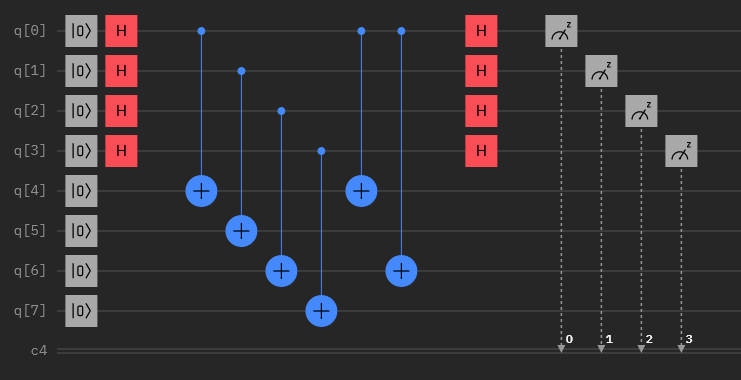
\includegraphics[width=0.7\textwidth]{0101.png}
    \caption{Simon's Algorithm Circuit with $ c = 0101 $}
\end{figure}

\section*{Part 2}


\subsection*{\text{a)}}

"Majority voting" is an error correction technique used in classical computation where the same data is replicated across multiple, redundant systems. When a read operation occurs, all copies are read, and the value that appears most frequently (the majority) is considered the correct value. This method is effective in correcting single errors in the data, assuming that the majority of the copies are correct, like sending $111$ for just a single bit $1$ even if it will be recieved as $101$, since the majority is still 1, it will be considered as $1$, so in this way the chance of error, which is higher for just one bit, is reduced.

In quantum computing, majority voting as it is classically understood cannot be directly applied because of the non-cloning theorem, which states that it is impossible to create an identical copy of an arbitrary unknown quantum state. Furthermore, bit flips are not the only possile errors in quantum computing, like phase-flips. 

\subsection*{\text{b)}}
My id is 2448546, and sum of its digits is 33. The phase gate will be $ P(\frac{46 \pi}{33}) $. The angle $ \theta $ is $4.379$ radians, and the cosine of this angle is $ -0.327 $. When these gates are applied respectively, after first H gate, we have $ | \psi \rangle = \frac{1}{\sqrt{2}} (|0\rangle + |1\rangle) $. After the phase gate, we have $ | \psi \rangle = \frac{1}{\sqrt{2}} (|0\rangle + e^{i \theta} |1\rangle) $. Then again after the H gate, we have $ | \psi \rangle = \frac{1}{2} (1 + e^{i \theta}) |0\rangle + \frac{1}{2} (1 - e^{i \theta}) |1\rangle $. From there, the probability of measuring $ |0\rangle $ is 0.336 and the probability of measuring $ |1\rangle $ is 0.664. When I run this with the simulator, the results are similar to the expectations, 0.335 and 0.665, as follows:

\begin{figure}[H]
    \centering
    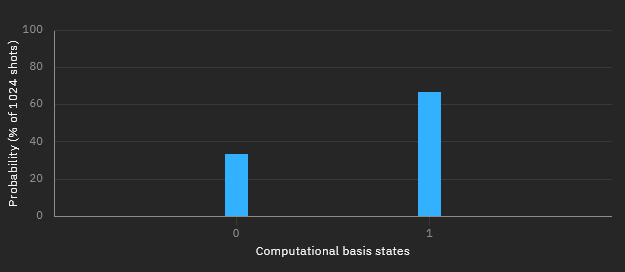
\includegraphics[width=0.8\textwidth]{simulator.png}
    \caption{Results of the circuit with the simulator}
\end{figure}

\newpage

\subsection*{\text{c)}}

Here is the first circuit and its result:

\begin{figure}[H]
    \centering
    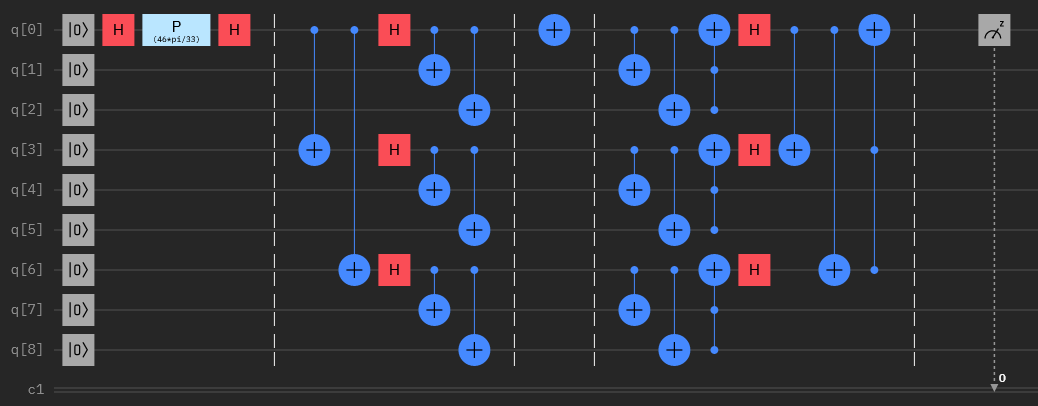
\includegraphics[width=0.9\textwidth]{shor1.png}
    \caption{The first circuit}
\end{figure}

\begin{figure}[H]
    \centering
    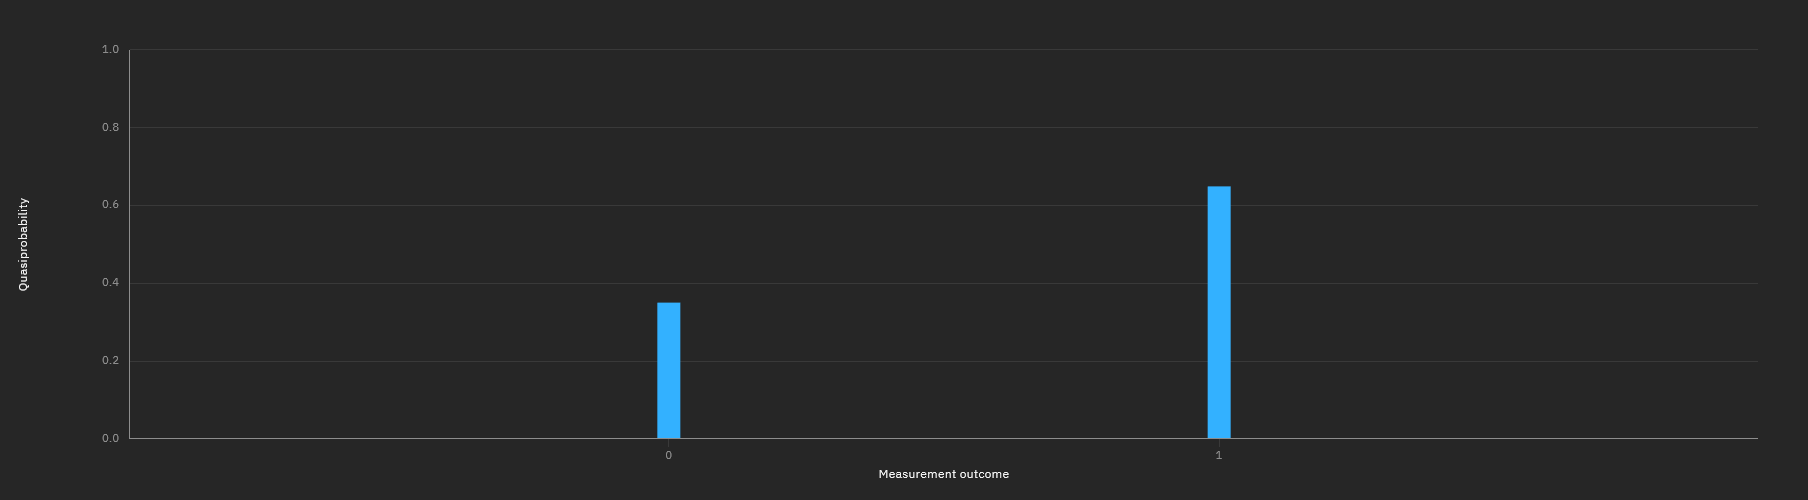
\includegraphics[width=0.9\textwidth]{shor1R.png}
    \caption{The result of the first circuit}
\end{figure}

Firstly, I initialized the first qubit with the value I found on the previous part. Then, in the first area separated with barriers, error encoding is implemented, then the error is injected, and finally, error decoding is implemented on the last separated area.

With these steps of error correction, the new results are 0.351 for $ |0\rangle $ and 0.649 for $ |1\rangle $. The circuit seems correct, yet someshow the results are slightly worse than the one without error correction on the previous part.

\newpage

Here is the second circuit and its result:

\begin{figure}[H]
    \centering
    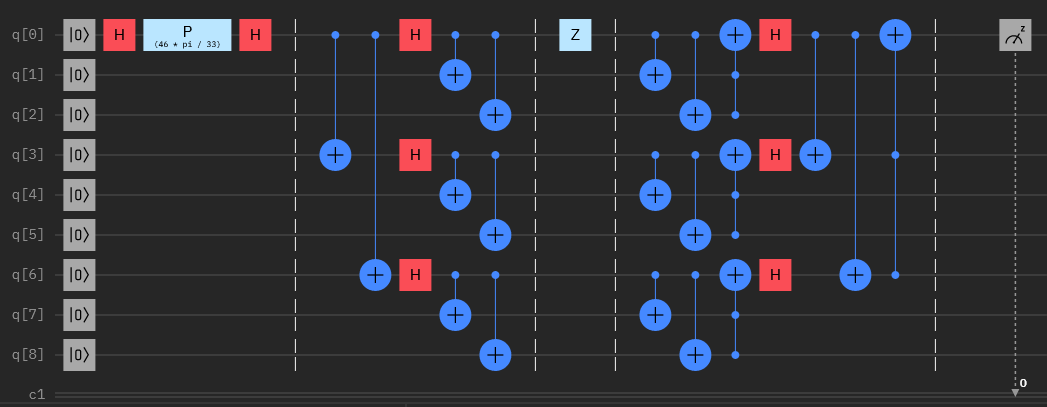
\includegraphics[width=0.9\textwidth]{shor2.png}
    \caption{The second circuit}
\end{figure}

\begin{figure}[H]
    \centering
    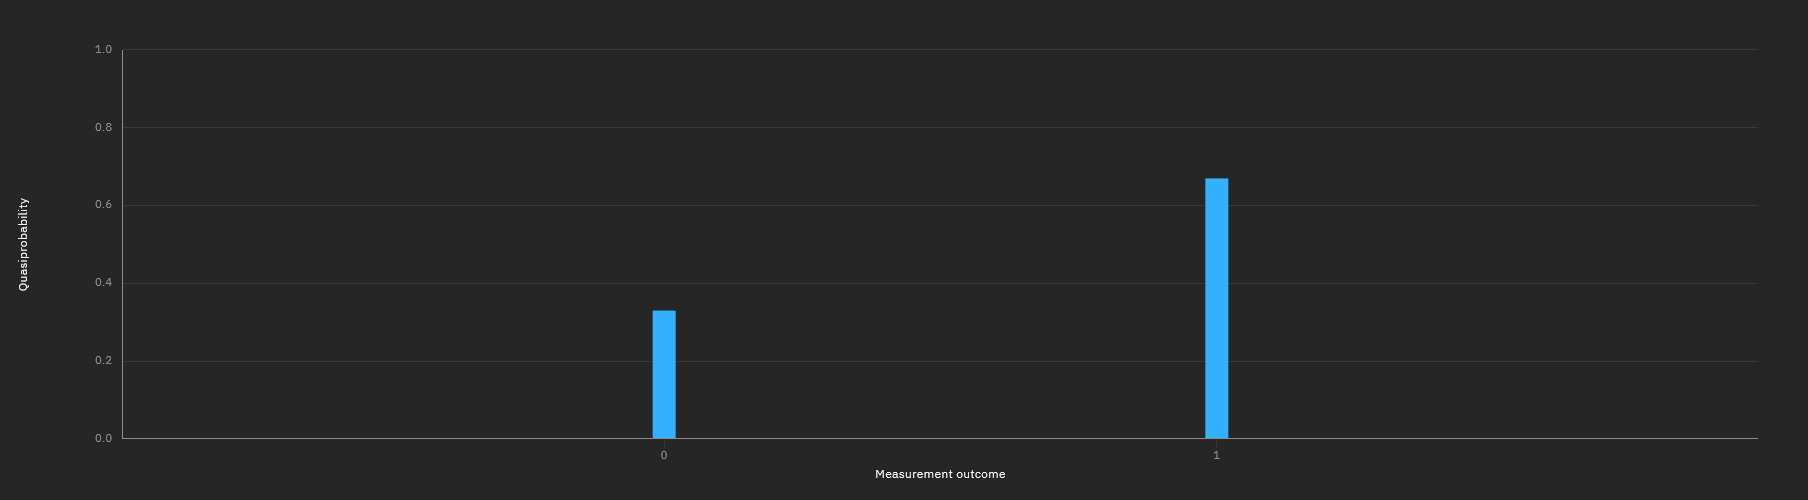
\includegraphics[width=0.9\textwidth]{shor2R.png}
    \caption{The result of the second circuit}
\end{figure}

The encoding and decoding are the same as the previous circuit, this time instead of NOT gate there is a Z gate. The results are 0.33 and 0.67, which are slightly better than the previous circuit and closer to the expected results.

\newpage

Here is the third circuit and its result:

\begin{figure}[H]
    \centering
    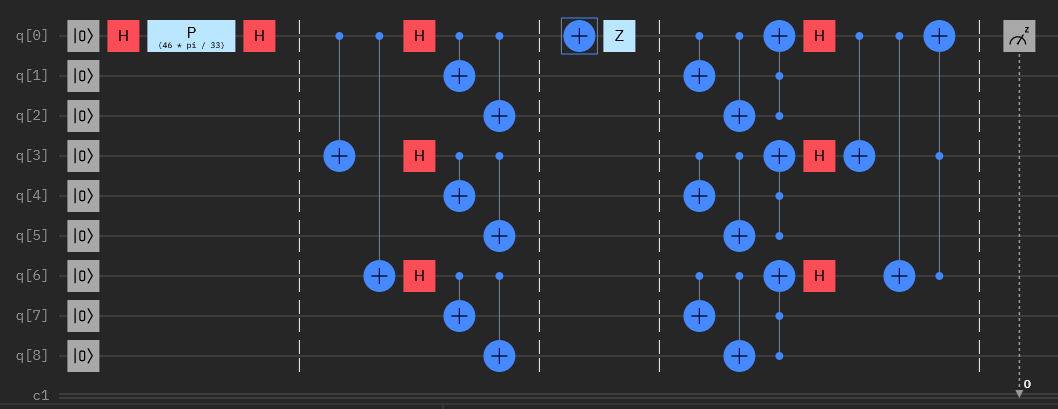
\includegraphics[width=0.9\textwidth]{shor3.png}
    \caption{The third circuit}
\end{figure}

\begin{figure}[H]
    \centering
    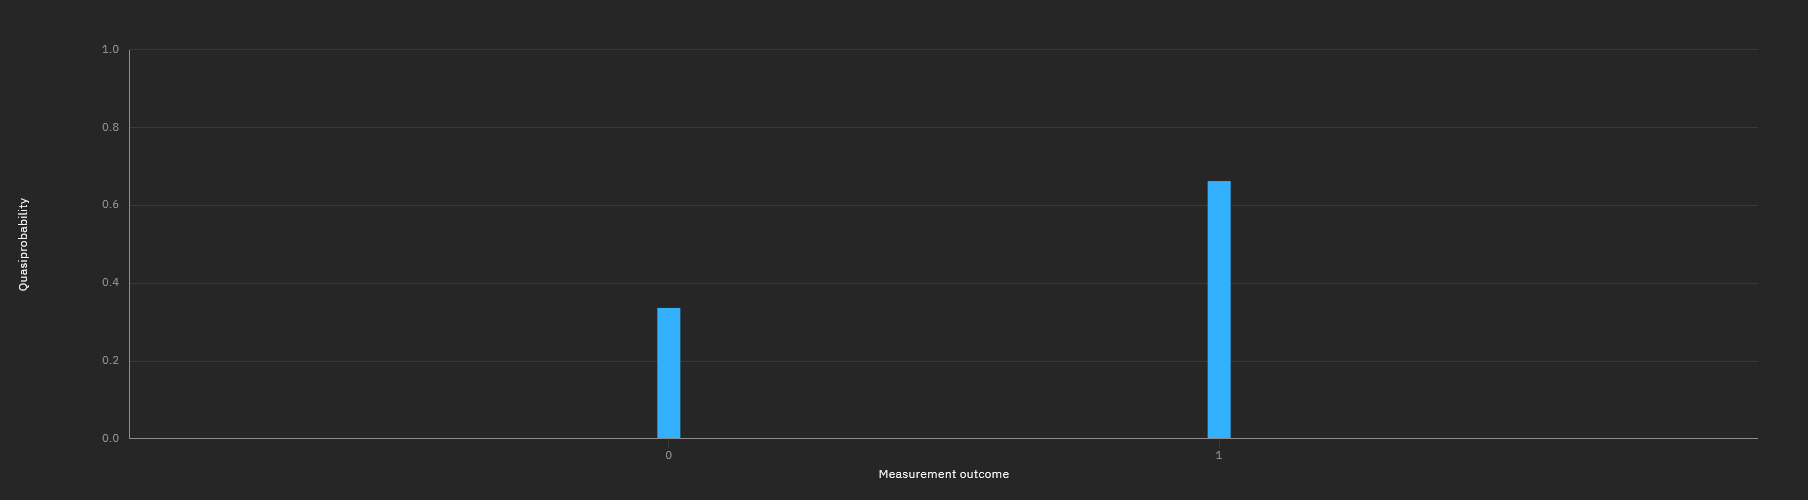
\includegraphics[width=0.9\textwidth]{shor3R.png}
    \caption{The result of the third circuit}
\end{figure}

The encoding and decoding are the same as the previous circuit, this time both of the gates are injected in the error area. The results are 0.337 and 0.663, which are the best results among the three circuits, and the closest to the expected results.


\end{document}
